\section{8\:\TeV\: Studies}
\label{app:toptaggerefficiency8TeV}

In this Appendix we compare the efficiency and fake rates of the top taggers measured in the 8 TeV data with the ones predicted by the simulations. The same procedure described is Sec. \ref{subsec:sel_toptag_resolved} has been used. An overall good agreement between data and prediction is seen.

 \begin{figure}[htbp]
	\centering
	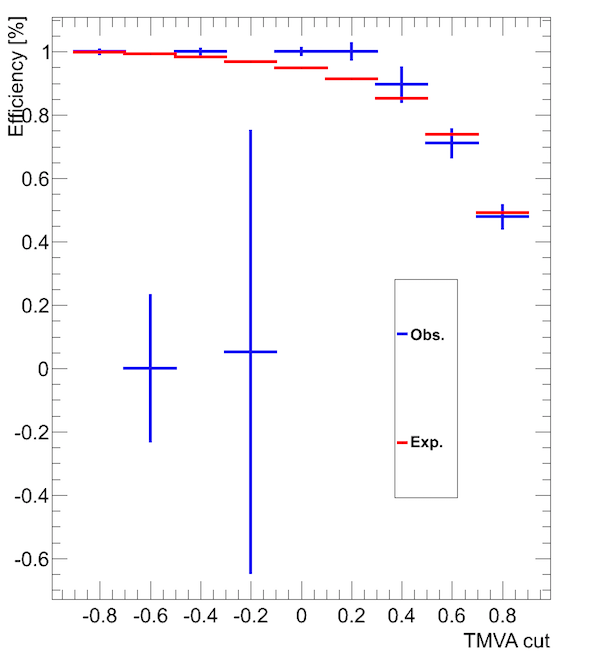
\includegraphics[width=0.48\textwidth]{figures/TOPRESOLVEDTAGGER/c_eff.png}\\
	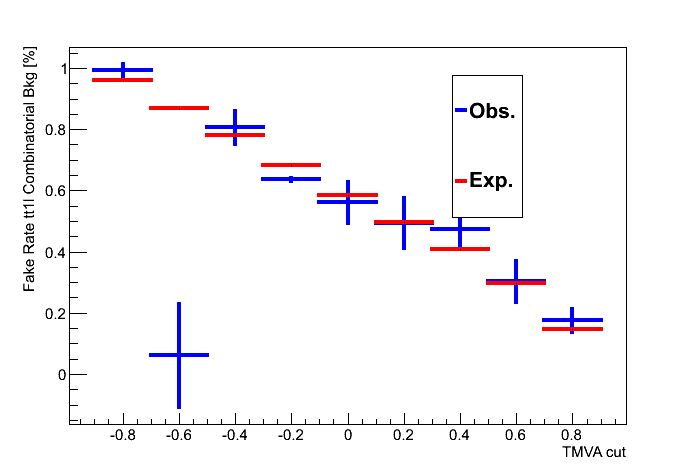
\includegraphics[width=0.48\textwidth]{figures/TOPRESOLVEDTAGGER/c_fr1.png}
	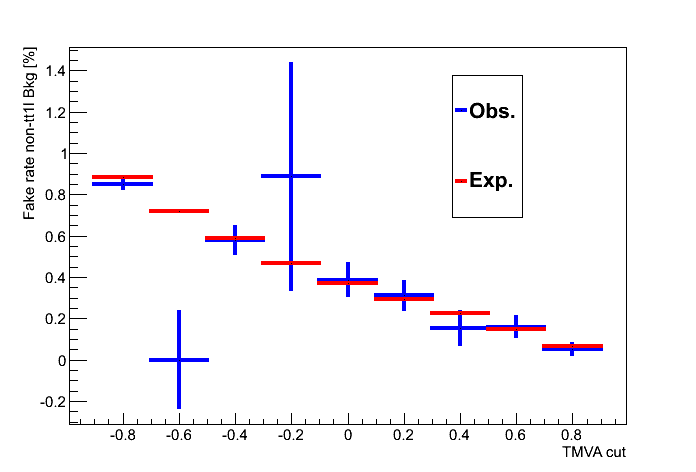
\includegraphics[width=0.48\textwidth]{figures/TOPRESOLVEDTAGGER/c_fr2.png}
	\caption{Signal efficiency (top),  combinatorial background fake rate (bottom left), and non-$\ttbar(1\Lep)$ background fake rate (bottom right) in 8 TeV data (blue) and mc (red) as function of the MVA threshold. The procedure to estimate those quantities has been described in the text. For the few bins where data and the predictions are consistent we noticed that Roofit has not reached convergence. \textcolor{red}{TO BE UNDERSTOOD}}
	\label{fig:roofitresults13TeV}
\end{figure}